%_________________________________________Heading_______________________________________________%

\documentclass[11pt]{article}
% #1-Asignatura
% #2-Curso
% #3-Nombre
% #4-Link
% #5-Foto

\newcommand{\portada}[5]{
    \begin{titlepage}
        \begin{center}
            \vspace*{0.5cm}
            
            % Titulo con #1 lo mas grande posible
            {\Huge \textbf{#1}}

            
            \vspace{0.5cm}
            \LARGE
            Curso #2 
            
            \vspace{1cm}
            
            \Huge{\textbf{Grupo Viterbi}}

            \vspace{1cm}
            
\includegraphics[width=0.6\textwidth]{assets/Img/UGR-Logo.png}
            
            \vspace{0.5cm}

            \huge
            PRÁCTICA 5- PROGRAMACIÓN DINÁMICA
            
            \Large
            \vspace{1cm}
            \textbf{Integrantes:}  \\ 
             % Array con los nombres de los integrantes y el correo
             \begin{center}
                \begin{tabular}{c c }
                    \textbf{Miguel Ángel De la Vega Rodríguez} & miguevrod@correo.ugr.es \\
                    \textbf{Alberto De la Vera Sánchez} & joaquinrojo724@correo.ugr.es \\
                    \textbf{Joaquín Avilés De la Fuente} & adelaveras01@correo.ugr.es \\
                    \textbf{Manuel Gomez Rubio} & e.manuelgmez@go.ugr.es \\
                    \textbf{Pablo Linari Perez} & e.pablolinari@go.ugr.es
                \end{tabular}
             \end{center}
            \vspace{0.8cm}
            
            
            \large
             \vspace{1cm}
            Facultad de Ciencias UGR\\
            Escuela Técnica Ingeniería Informática UGR\\
            Granada\\
            #2 
            
        \end{center}
    \end{titlepage}
}



\usepackage{assets/formulas}
\usepackage{float}
\hbadness=10000 % Suppress Underfull \hbox warnings

%_________________________________________Indice:_______________________________________________%
\begin{document}                                                
\portada{Algorítmica}{2023-2024}{Miguel Ángel De la Vega Rodríguez}{https://github.com/Miguevrgo/}{github.png}

\tableofcontents % Índice

\newpage %Salto de pagina tras el Indice

%________________________________________Documento:_____________________________________________%
\section{Participación}
\begin{itemize}
    \item \textbf{Miguel Ángel De la Vega Rodríguez:} 20\%
    \begin{itemize}
        \item Plantilla y estructura del documento \LaTeX
        \item Cómputo de la eficiencia de los algoritmos (Resultados y Ajuste)
    \end{itemize}
    \item \textbf{Joaquín Avilés De la Fuente:} 20\%
    \begin{itemize}
        \item Descripción del Objetivo de la pŕactica
        \item Diseño del estudio
    \end{itemize}
    \item \textbf{Alberto De la Vera Sánchez: } 20\%
    \item \textbf{Manuel Gomez Rubio} 20\%
    \item \textbf{Pablo Linari Perez:} 20\%
\end{itemize}

\section{Equipo de trabajo}

\begin{itemize}
    \item \textbf{Miguel Ángel De la Vega Rodríguez:} (Ordenador donde se ha realizado el computo)
        \begin{itemize}
            \item AMD Ryzen 7 2700X 8-Core
            \item 16 GB RAM DDR4 3200 MHz
            \item NVIDIA GeForce GTX 1660 Ti 
            \item 1 TB SSD NvMe 
        \end{itemize}
\end{itemize}

\section{Objetivos}
    En esta práctica, se han implementado los siguientes algoritmos de ordenación: \textbf{quicksort, mergesort, heapsort, inserción, burbuja,}
    y \textbf{selección}. Además, se han implementado los algoritmos de \textbf{Floyd}, que calcula el costo del camino mínimo entre cada par de nodos 
    de un grafo dirigido, de \textbf{Fibonacci}, que calcula los números de la sucesión de Fibonacci , y de \textbf{Hanoi}, que resuelve el famoso 
    problema de las torres de Hanoi. Se ha aplicado la siguiente metodología:
    \begin{itemize}
        \item En primer lugar, aunque tenemos la eficiencia teórica de estos algoritmos, se realizarán los calculos necesarios para demostrar
        como se obtiene dicha eficiencia utilizando los distintos métodos estudiados en teoría. \\
        
        \item En segundo lugar, se pasará al estudio empírico de los algoritmos de ordenación de vectores para distintos tipos de datos, es decir, 
        para datos tipo \textbf{int}, \textbf{float}, \textbf{double} y \textbf{string}. Posteriormente, se creará las gráficas para
        cada algoritmo en las que visualizaremos el tiempo de ejecución en función del tamaño del vector y del tipo de dato. Finalmente 
        para esta parte, se hara un calculo de \textbf{eficiencia híbrida} que se basa en ajustar la gráfica obtenida a la función de su eficiencia
        teórica por mínimos cuadrados, obteniendo por tanto los literales de dicha función que ajustan la gráfica.\\
        
        \item En tercer lugar, se hará el estudio de los otros tres algoritmos de forma similar, es decir, se estudiará la eficiencia
        de estos de modo empírica, cuyo estudio se mostrará en las gráficas, y se calculará la eficiencia híbrida de estos, a partir
        de la eficiencia teórica.\\     
    \end{itemize}
\section{Diseño del estudio}
    % Esta variable indica el algoritmo escogido para el estudio en varios ordenadores
    \newcommand{\mivar}{ordenación de vectores quicksort}
    Los estudios empíricos han sido realizados en el ordenador con las características mencionadas anteriormente.
    Además, hemos realizado el estudio empírico de forma aislada para el algoritmo de ordenación de vectores
    quicksort en los distintos ordenadores de los participantes del grupo para ver como afectan las características
    hardware de cada ordenador en el tiempo de ejecución, cuyas gráficas se mostrarán en la sección de Algoritmos. \\
    En ambos casos se ha hecho uso del sistema operativo Linux, concretamente de Debian, y se ha utilizado el
    compilador gcc para la compilación de los programas  con el flag -Og para la optimización.
    \subsection{Algoritmos de ordenación de vectores}
    Para la facilitación del estudio empírico de los algoritmos se ha hecho uso de varios scripts, entre ellos:
    \begin{itemize}
        \item \textbf{[AutoCompile.sh]} Este script se encarga de compilar todos los ficheros en una misma carpeta con las mismas
        opciones de compilación, para garantizar la máxima igualdad posible entre cada algoritmo y organizar la estructura de 
        ficheros.
        \item \textbf{[AutoFinal.sh]} Este script es el encargado de ejecutar todos los algoritmos varias veces con las opciones respectivas para cada uno,
        el resultado se pasa por un programa AutoMedia.py que se encarga de realizar la media de las ejecuciones de los algoritmos,
        este resultado es guardado en una carpeta llamada Resultados de la que posteriormente el mismo script genera las graficas
        de cada algoritmo.
        \item \textbf{[AutoIndividual.sh]} Este script es como el descrito previamente pero unicamente ejecuta un script, esto ha sido útil para hacer
        pruebas sin la necesidad de esperar la gran cantidad de tiempo que requiere la ejecución de todos los algoritmos.
    \end{itemize}
    
\section{Algoritmos}
Esta sección esta dedicada a mostrar los resultados obtenidos en el estudio de los algoritmos,
la estructura seguida para mostrar los resultados consiste en mostrar, para cada algoritmo, los tiempos 
de ejecución, junto con las gráficas obtenidas y los ajustes correspondientes. Previo a ello, se analizará
en cada caso teoricamente la eficiencia prevista para cada algoritmo.

\subsection{Burbuja}
\begin{figure}[H]
    \begin{minipage}{0.5\textwidth}
        \centering
        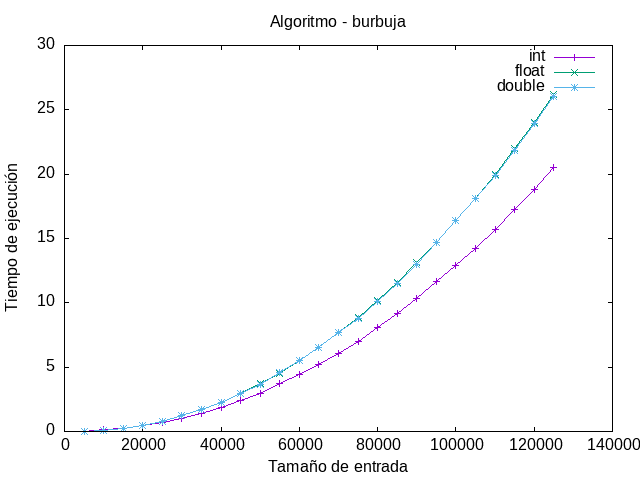
\includegraphics[width=\linewidth]{assets/Img/burbuja.png}
        \caption{Ejecución algoritmo burbuja}
        \label{fig:burbuja}
    \end{minipage}%
    \begin{minipage}{0.5\textwidth}
        \centering
        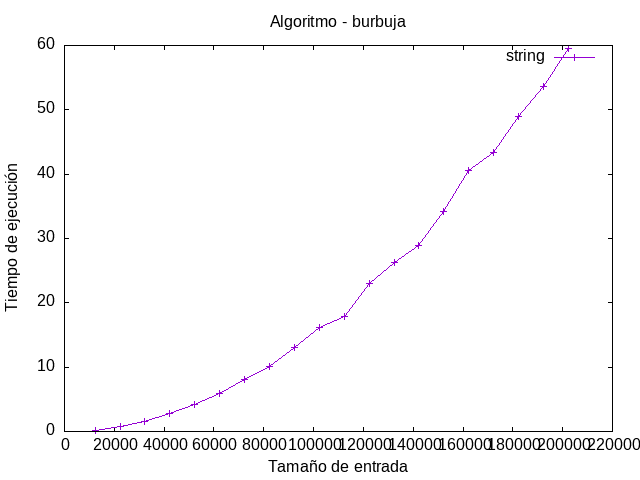
\includegraphics[width=\linewidth]{assets/Img/burbujastring.png}
        \caption{Ejecución algoritmo burbuja con string}
        \label{fig:burbujastring}
    \end{minipage}
\end{figure}
\subsection{Seleccion}
\begin{figure}[H]
    \begin{minipage}{0.5\textwidth}
        \centering
        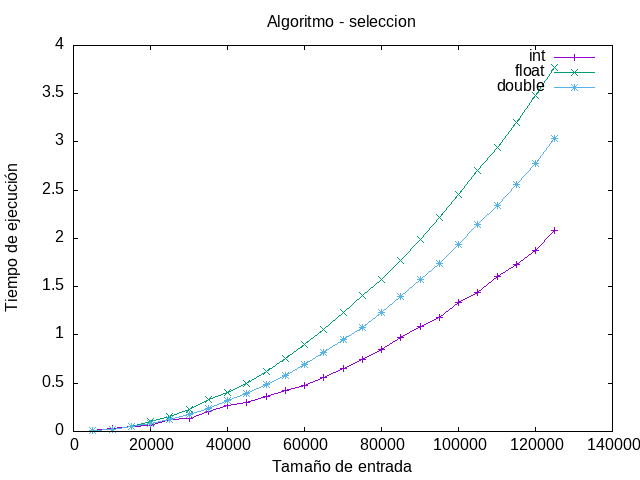
\includegraphics[width=\linewidth]{assets/Img/seleccion.png}
        \caption{Ejecución algoritmo seleccion}
        \label{fig:seleccion}
    \end{minipage}%
    \begin{minipage}{0.5\textwidth}
        \centering
        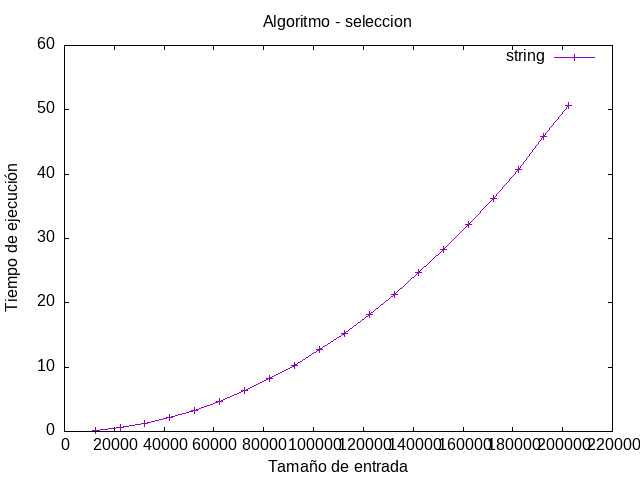
\includegraphics[width=\linewidth]{assets/Img/seleccionstring.png}
        \caption{Ejecución algoritmo seleccion con string}
        \label{fig:seleccionstring}
    \end{minipage}
\end{figure}

\subsection{Inserción}
\begin{figure}[H]
    \begin{minipage}{0.5\textwidth}
        \centering
        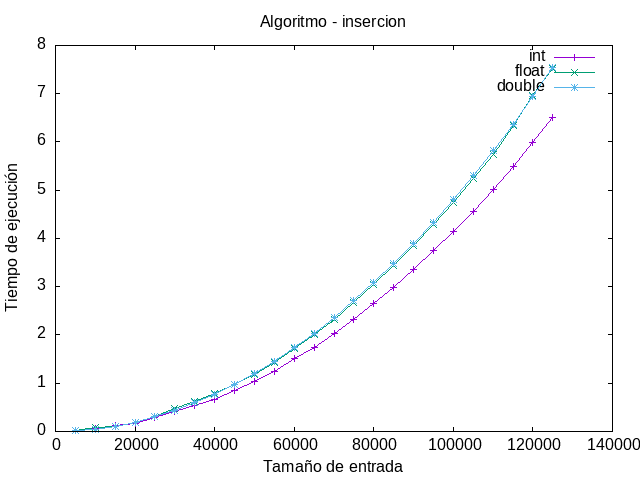
\includegraphics[width=\linewidth]{assets/Img/insercion.png}
        \caption{Ejecución algoritmo insercion}
        \label{fig:insercion}
    \end{minipage}%
    \begin{minipage}{0.5\textwidth}
        \centering
        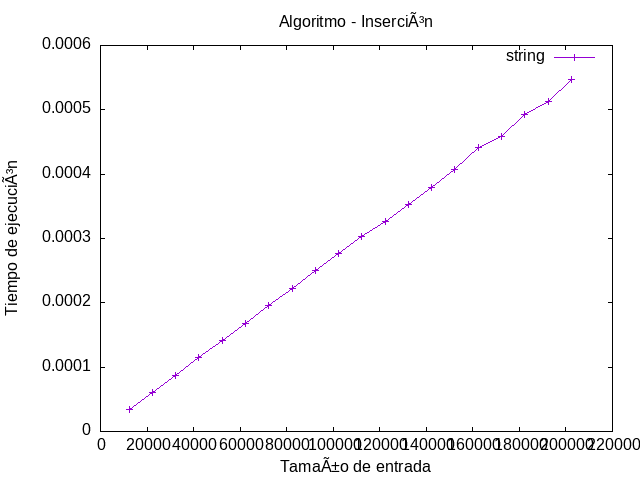
\includegraphics[width=\linewidth]{assets/Img/insercionstring.png}
        \caption{Ejecución algoritmo inserción con string}
        \label{fig:insercionstring}
    \end{minipage}
\end{figure}
\subsection{Hanoi}
\begin{figure}[H]
    \centering
        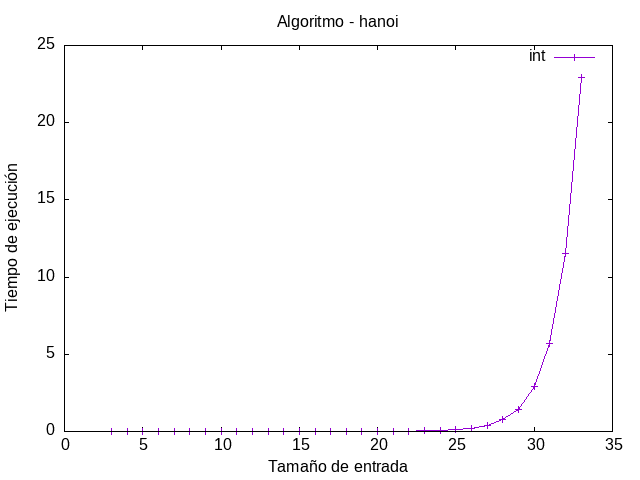
\includegraphics[width=0.5\linewidth]{assets/Img/hanoiint.png}
        \caption{Ejecución algoritmo Hanoi}
        \label{fig:hanoi}
\end{figure}
\subsection{Fibonacci}
\begin{figure}[H]
    \centering
        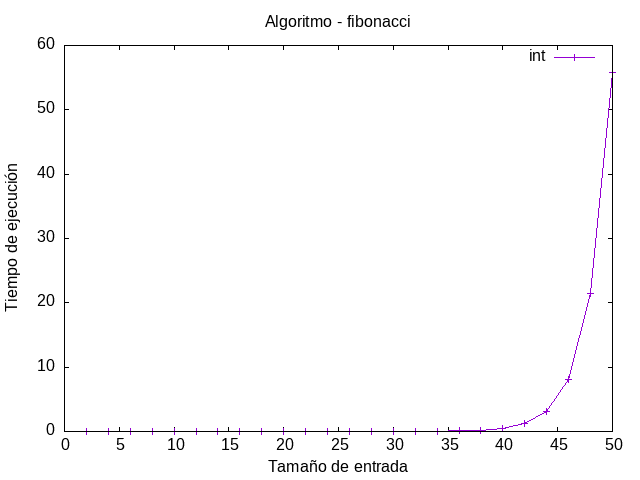
\includegraphics[width=0.5\linewidth]{assets/Img/fibonacciint.png}
        \caption{Ejecución algoritmo Fibonacci}
        \label{fig:fibonacci}
\end{figure}
\subsection{Floyd}
\begin{figure}[H]
    \centering
        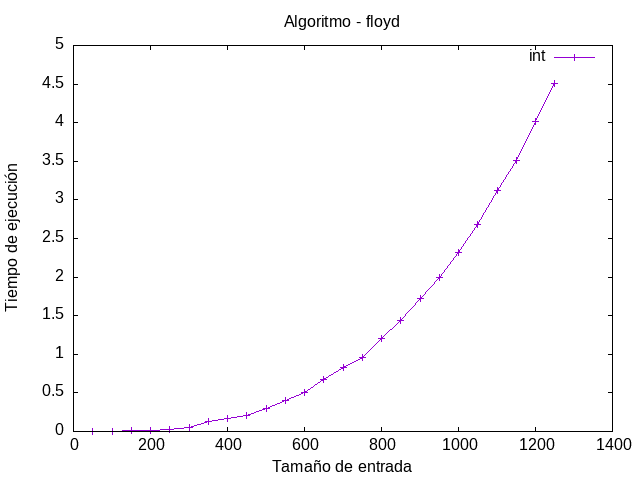
\includegraphics[width=0.5\linewidth]{assets/Img/floydint.png}
        \caption{Ejecución algoritmo Floyd}
        \label{fig:floyd}
\end{figure}
\section{Conclusiones}

\end{document}